\documentclass[12pt, a4paper]{article}

% page layout packages
\usepackage{fancyhdr}
\usepackage[margin=1in]{geometry}
\usepackage{titlesec}

% mathematical packages
\usepackage{amsthm}
\usepackage{leftidx}
\usepackage{mathptmx}

% table enhancement packages
\usepackage{booktabs}
\usepackage{diagbox}
\usepackage{ragged2e}
\usepackage{tabularx}

% graphics packages
\usepackage{graphicx}
\usepackage{tikz}
\usetikzlibrary{shapes.geometric, arrows}

% text formatting packages
\usepackage{latexsym}
\usepackage[normalem]{ulem}
\usepackage{xcolor}

\newcommand{\todo}[2]{\textbf{\color{blue}[TODO \##1] #2}\par}
\newcommand{\done}[2]{\textbf{\color{gray}\sout{[TODO \##1] #2}}\par}

\setcounter{secnumdepth}{4}

\parindent 0pt
\parskip 5pt
\pagestyle{fancy}

\fancyhead[L]{Consensus}
\fancyhead[R]{COMP90020 Distributed Algorithms}
\fancyfoot[L]{Semester 1, 2020}
\fancyfoot[C]{}
\fancyfoot[R]{\thepage}
\fancypagestyle{firststyle}{%
  \fancyhf{}
  \fancyfoot[L]{Semester 1, 2020}
  \fancyfoot[R]{\thepage}
  \renewcommand{\headrulewidth}{0pt}
}
\renewcommand{\headrulewidth}{0.4pt}
\renewcommand{\footrulewidth}{0.4pt}
\renewcommand{\arraystretch}{1.2}

\title{{An Overview of Consensus with a Detailed Comparison between Paxos and Raft}}
\author{
  Qifan Deng \\
  \texttt{\small qifand@student.unimelb.edu.au}
  \and
  Zhaofeng Qiu \\
  \texttt{\small zhaofengq@student.unimelb.edu.au}
  \and
  Alan Ung \\
  \texttt{\small alanu@student.unimelb.edu.au}
  \and
  Yangzhe Xie \\
  \texttt{\small yangzhex@student.unimelb.edu.au}
  \and
  Min Zhao \\
  \texttt{\small zhaomz1@student.unimelb.edu.au}
}
\date{Semester 1, 2020}

\newtheorem*{assumption*}{\assumptionnumber}
\providecommand{\assumptionnumber}{}
\makeatletter
\newenvironment{assumption}[2]
 {
  \renewcommand{\assumptionnumber}{Assumption #1}
  \begin{assumption*}
  \protected@edef\@currentlabel{#1}
 }
 {
  \end{assumption*}
 }
\makeatother
\newcommand{\asref}[2]{\ref{#1}}

% https://tex.stackexchange.com/questions/60209
\titleformat{\paragraph}
{\normalfont\normalsize\bfseries}{\theparagraph}{1em}{}
\titlespacing*{\paragraph}
{0pt}{3.25ex plus 1ex minus .2ex}{1.5ex plus .2ex}
\begin{document}
\maketitle
\thispagestyle{firststyle}

%%%%%%%%%%%%%%%%%%%%%%%%%%%%%%%%%%%%%%%%%%%%%%%%%%%%%%%%%%%%%%%%%%%%%%%%%%%%%%%%

\section{Abstract}
Consensus is a core problem in distributed computing, relevant to a wide range of applications. We provide an overview of the literature surrounding the consensus problem and present a comparative analysis of different approaches to solving it. Thereafter, we focus specifically on \textit{Paxos} and \textit{Raft}. We implement a distributed key-value database in Java using the Raft algorithm as its core as a case study. We describe an enhancement to the Raft algorithm which we implement before concluding with a discussion on the application domains and future directions of consensus.

% Assuming the network is unreliable, consensus algorithms are designed to achieve agreement on a single data value among distributed systems. Consensus algorithms can be broadly classed as following one of two main approaches---voting-based consensus and proof-based consensus. Based on their respective advantages, they are used in various fields. In this report, we mainly focus on introducing the Raft and Paxos algorithms and give a detail implementation with raft algorithm on distributed key-value based database application.

% In a distributed system, the instructions between servers should be consistent. When one of the servers receives a single instruction from the client, it must communicate with other servers to ensure that all servers receive the same instructions in the same order. This will enable all servers to produce consistent results that look like one machine. This type of problem is defined as a consensus problem which is a key aspect on distributed system’s construction. There are many consensus algorithms used to solve the consensus problem. In this report, we mainly focus on introducing the Raft and Paxos algorithms and give a detail implementation with raft algorithm on distributed key-value based database application.

\textbf{Keywords}: Distributed consensus, Raft, Paxos, State machine replication, Key-value database

%%%%%%%%%%%%%%%%%%%%%%%%%%%%%%%%%%%%%%%%%%%%%%%%%%%%%%%%%%%%%%%%%%%%%%%%%%%%%%%%

\section{Introduction}

Achieving agreements among remote processes in a distributed system is a fundamental problem relevant to a wide range of applications \cite{fischer1985impossibility, kshemkalyani_singhal_2008}. Indeed, many common tasks---such as coordinating access to shared resources, electing a leader and achieving agreement on message delivery order---share the core requirement for processes to communicate and negotiate with each other to establish a common understanding before taking further action \cite{kshemkalyani_singhal_2008, coulouris2005distributed}.

The \textit{consensus} problem generalises these tasks to ask how a collection of processes can agree on a value $v$, no matter the domain from which $v$ may be taken \cite{coulouris2005distributed}. Due to issues such as node failures and network unreliability, it can be difficult to achieve consistency among nodes in distributed computing or multi-agent systems \cite{coulouris2005distributed}. Therefore, the algorithms used to achieve consensus must take failures into consideration and aim to be as robust as possible.

This report first provides a formal definition of the consensus problem in \S\ref{sec:consensus-def}. We then discuss important fundamental models in \S\ref{sec:fundamental-models} which are important to consider when comparing and analysing different distributed algorithms. In doing so, we will discover that under a certain fundamental model, no algorithm can guarantee consensus under all circumstances.

To further motivate the consensus problem and expand on its aforementioned fundamentality to many applications, we discuss its relationship to a range of relevant tasks in \S\ref{sec:motivation}. A background survey of the literature is provided in \S\ref{sec:background} to provide an overview of different approaches to solving the problem of consensus. We provide a detailed comparative analysis between the two in \S\ref{sec:comparitive}, discussing the benefits and drawbacks of either algorithm.

We then focus on two algorithms by which to achieve consensus. \textit{Paxos} \cite{lamport1998part, lamport2001paxos} (detailed in \S\ref{sec:paxos}) has been the dominant consensus algorithm for much of the past two decades, underpinning most implementations of consensus \cite{ongaro2014search}. More recently, however, a contending consensus algorithm has been proposed. \textit{Raft} \cite{ongaro2014search} (detailed in \S\ref{sec:raft}) is purported by its authors to ``[produce] a result equivalent to (multi-)Paxos'' and be ``as efficient as Paxos'' yet ``more understandable'' and able to ``provide a better foundation for building practical systems.'' \cite{ongaro2014search}

Additionally, we detail our own implementation of the Raft algorithm as part of a key-value database application in \S\ref{sec:application}, bringing the algorithm into a concrete context. Finally, we discuss the application domains and future directions in \S\ref{sec:future}.

%%%%%%%%%%%%%%%%%%%%%%%%%%%%%%%%%%%%%%%%%%%%%%%%%%%%%%%%%%%%%%%%%%%%%%%%%%%%%%%%

\section{Problem Definition} \label{sec:consensus-def}

The consensus problem is defined with respect to a collection of $N$ processes which communicate by message passing. Every process $p_{i}$ $(i = 1, \ldots, N)$ begins in the \textit{undecided} state, in which they each propose a single value $v_{i} \in D$, where $D$ is a set of acceptable values \cite{coulouris2005distributed}.

The processes then exchange values with each other. During this phase, each process sets the value of its \textit{decision variable}, $d_i$ $(i = 1, \ldots, N)$, based on the information obtained from other processes. In doing so, they enter the \textit{decided} state, in which the decision variable may no longer change.

A consensus algorithm must satisfy the following conditions for every execution:

\begin{itemize}
  \item \textbf{Termination}: Each non-faulty process $p_i$ must eventually set
    $d_i$.
  \item \textbf{Agreement}: All non-faulty processes in the decided state
    must have the same value. If $p_{i}$ and $p_{j}$ are correct and have
    entered the decided state, then $d_{i} = d_{j}$ $(i, j = 1, \ldots, N)$.
  \item \textbf{Integrity/Validity}: If all non-faulty processes proposed
    the same value, then the decision variable of all non-faulty processes is
    that same value.
\end{itemize}

\subsection{Fault Tolerance}
A distributed system, by nature, requires communication between nodes throughout its operation. However, nodes are prone to failures which can present unintended behaviour if the system is not robust against such failures. Consensus algorithms are designed to
solve this issue by introducing a degree of fault tolerance to the system.

An algorithm is classed as \textit{Crash Fault Tolerant} (CFT) if it can operate throughout failures caused by process crashes or fail-stops. Additionally, an algorithm is classed as \textit{Byzantine Fault Tolerant} (BFT) if it can handle arbitrary faults, including those arising from malicious actions of an adversary.

Any BFT algorithm is also a CFT algorithm, since Byzantine failures encompass all possible faults in the system model. The hierarchy of different faults \cite{barborak1993consensus} is shown in Figure \ref{fig:aofc}.

\begin{figure}[htp]
  \centering
  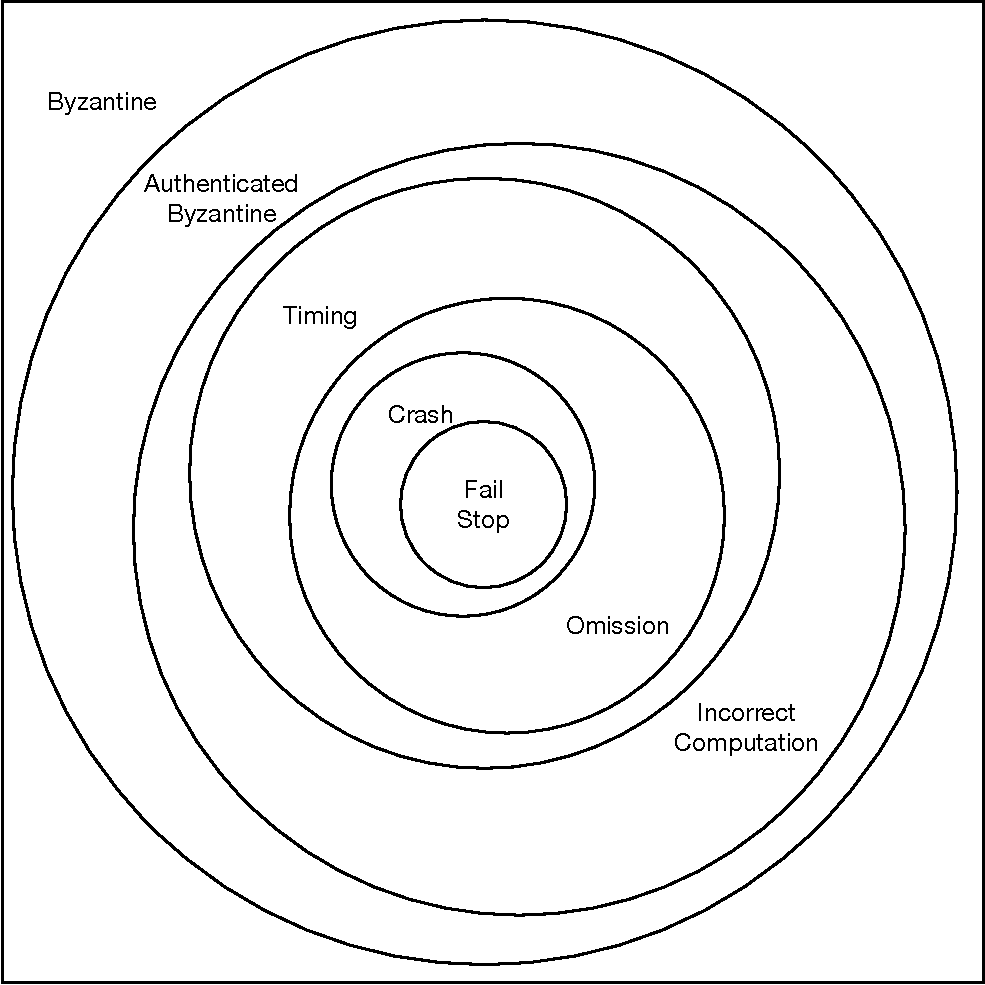
\includegraphics[width=0.5\textwidth]{img/AOFC.pdf}
  \caption{An ordered fault classification (Barborak et al.)}
  \label{fig:aofc}
\end{figure}

\subsection{Consensus Under Different Models of Computation} \label{sec:fundamental-models}
Solving the consensus problem varies in difficulty depending on the system model being considered. Different models assert different assumptions and thus, it is important to consider the impacts of such models on the consensus algorithms to be investigated.

\subsubsection{Synchronous and Asynchronous Systems}
\textit{Fundamental models} provide an ``abstract perspective'' for considering individual aspects of a distributed system \cite{coulouris2005distributed}. An \textit{interaction model} is a fundamental model concerned with communication and coordination between processes, including aspects such as process execution, message delivery and clock drift \cite{coulouris2005distributed}. Although it is difficult to set limits on these, considering ``two extremes of a spectrum'' gives rise to a pair of simple models---one with strong assumptions about time and the other with none \cite{coulouris2005distributed, hadzilacos1994modular}.

The \textit{synchronous} system model is defined by Hadzilacos and Toueg \cite{hadzilacos1994modular} to be one in which:

\begin{enumerate}
  \item Time taken by a process to execute a step has known upper and lower
    bounds.
  \item Every process has a local clock whose drift rate has a known bound.
  \item There is a known upper bound on message delay.
\end{enumerate}

These bounds are global across the entire system. A collection of processors connected by a communication bus is an example of a system which closely aligns to the synchronous model.

By contrast, the \textit{asynchronous} system model is one which makes no assumptions about time \cite{coulouris2005distributed, hadzilacos1994modular}. Namely, there are no bounds on process execution time or message transmission delay and clock drift rates may be arbitrarily fast or slow \cite{coulouris2005distributed}. This model is useful when considering systems such as the Internet \cite{coulouris2005distributed}.

The asynchronous model is more general than the synchronous counterpart. As such, it is more difficult to solve the consensus problem under the former than the latter. An algorithm which works under the asynchronous model will also work for the synchronous model.

The consensus problem is solvable under the synchronous model \cite{fischer1985impossibility, kshemkalyani_singhal_2008}. However, it has been shown by Fischer \cite{fischer1985impossibility} to be impossible to solve under the asynchronous model. No matter the protocol or algorithm, there is always a ``window of vulnerability'' during which the failure of processes or delay of messages prevents the system from reaching consensus by way of nontermination \cite{fischer1985impossibility}. Despite this, it should be noted that the impossibility arises from a worst-case scenario of low probability---in reality, process scheduling has aspects of randomness \cite{aguilera2010stumbling}. Thus, although it is not theoretically possible to guarantee consensus under the asynchronous model in all circumstances, consensus algorithms can still be implemented in practice.

\subsection{CAP Theorem and Consensus Algorithms}
\label{sec:cap-theorem}
The CAP theorem \cite{brewer2012cap} states that in a distributed system,
it is impossible for an algorithm to provide more than two of these three properties:
\begin{itemize}
	\item \textbf{Consistency (C)}: All data backups in the distributed system have
    the same value at the same time.
	\item \textbf{Availability (A)}: After some nodes in the cluster fail, the entire
    cluster can still respond to client read and write requests. However, there
    is no guarantee that the data produced is most up-to-date.
	\item \textbf{Partition tolerance (P)}: The system continues to operate despite
    delayed, lost or dropped messages on the network.
\end{itemize}

\subsubsection{Consistency and Partition-Tolerance}
Algorithms like Raft and Paxos sacrifice availability to achieve partition-tolerance and consistency. Nodes in clusters that guarantee consensus can recover from partitions and maintain consistency, but the smaller part not in the majority partition (not in the quorum) will not send responses if partition problem happens. Hence the availability is compromised in consensus algorithms.

%%%%%%%%%%%%%%%%%%%%%%%%%%%%%%%%%%%%%%%%%%%%%%%%%%%%%%%%%%%%%%%%%%%%%%%%%%%%%%%%

\section{Motivation}
\label{sec:motivation}

The consensus problem is key to many problems in distributed computing, making effective solutions to it highly desirable \cite{fritzke2001consensus}. To motivate consensus in context, related problems—highlighting useful applications in distributed computing—are discussed in this section. Below, we discuss four issues related to consensus problem; namely reliable multicast, membership protocol (failure detection), leader election and mutual exclusion. The consensus problem unifies and generalises these problems. In practice, this means that the following issues can be solved with the aid of consensus.

\subsection{Reliable Multicast}
Multicast is a form of group communication in which a single message is sent from one process to a \textit{group} of processes in a manner which is usually transparent to the sender \cite{coulouris2005distributed}. A \textit{reliable} multicast operation is one which guarantees that processes are consistent not only on the set of messages they deliver but also on the order of message deliveries \cite{fritzke2001consensus}. Different ordering classifications exist, as detailed below \cite{garcia1991ordered}.

\begin{itemize}
  \item \textbf{Single source ordering}: If messages are from the same source
  site, and they are sent to the same multicast group, then they should be
  received by all target processes in the same order.
  \item \textbf{Multiple source ordering}: If messages are from different
  source sites, and they are sent to the same multicast group,
  then they should be received by all target processes in the same order.
  \item \textbf{Multiple group ordering}: If two messages are from different
  source sites, and they are sent to different but overlapping multicast groups,
  they should be received by all target processes in the same order.
\end{itemize}

Many applications in distributed computing (such as banking, stock trading and e-commerce) require consistent message ordering between processes. Moreover, ordered communication can simplify the design of distributed applications and reduce the potential for bugs relating to synchronisation or concurrency \cite{garcia1991ordered}. This problem is closely tied to the problem of consensus, illustrating how consensus is central to useful applications.

\subsection{Membership/Failure Detection}
Since it is impossible to definitively distinguish between a crashed process and a slow one under the asynchronous system model, it is impossible to design a deterministic consensus algorithm under the asynchronous model, even in the case of a single process crash failure \cite{fischer1985impossibility}. Under the asynchronous model, the problems of failure detection and consensus are one and the same. This impossibility prompted many researchers to propose a minimum set of assumptions. As long as these assumptions are satisfied by the asynchronous distributed system, the consensus problem can be solved as well. The unreliable fault detector is the solution to this challenge \cite{chandra1996unreliable}.

Every process has a list of processes that are suspected to have crashed. This may be inaccurate by way of failing to include a process which has crashed or including one which is indeed still running. When process $p_{i}$ suspects that process $p_{j}$ crashed, we say that $p_{i}$ suspects $p_{j}$. Errors of the failure detector are typically defined by two properties:

\begin{itemize}
  \item \textbf{Completeness}: In the end, crashed processes should be suspected.
  \item \textbf{Accuracy}: Limit wrong suspicion of well-running processes.
\end{itemize}

Chandra and Toueg \cite{chandra1996unreliable} defined several classes of failure detectors. One of them is named as $\diamond$S with following two properties:

\begin{itemize}
  \item \textbf{Strong completeness}: Ultimately, all crashed processes are constantly suspected by every well-running process.
  \item \textbf{Eventual weak accuracy}: Ultimately, a well-running process never suspects a majority of well-running processes.
\end{itemize}

In practice, if a process does not receive a message response before the timeout occurs, the sending process suspects that the message receiving process has crashed. This can satisfy strong completeness. However, there is no guarantee of accurate process crash detection. This problem is of considerable interest with respect to consensus, as solving consensus under the asynchronous model would solve this as well. However, as previously mentioned, Fischer \cite{fischer1983consensus} has shown this to be impossible.

\subsection{Leader Election}
Leader election involves selection of a leader in a group of processes and reaching agreement regarding which process the leader is. A leader is the coordinator among processes and there can only be one leader at a time. In a distributed system, each node would need to exchange messages with other nodes in the network to make a decision without a leader. However, this method of communication between nodes is time-consuming, and when consistency among all nodes is required, coordination between nodes becomes difficult. Therefore, selecting a leader to manage the access of shared resources is desirable for efficiency. The implementation of a leader election should follow two basic properties \cite{nugraheni2009formal}:

\begin{itemize}
  \item \textbf{Safety}: There will never be two or more leaders at the same time.
  \item \textbf{Liveness}: The election algorithm always ends, and each process knows the leader who is ultimately elected.
\end{itemize}

In the leader election process, the leader is usually selected according to some criteria, such as the node with the largest identifier  \cite{effatparvar2010improved}. After the leader is elected, the node will reach a state called \textit{termination}. There are two such termination states, namely the elected state and the non-elected state. Once a node reaches its termination state, it always maintains that state. Moreover, when the leader fails, the leader election mechanism dynamically elects a new leader. The problem of leader election is closely tied to consensus---if nodes can agree on a value in general, they can agree on a process being the leader.

\subsection{Mutual Exclusion}
Distributed processes need to coordinate access to shared resources to prevent race conditions. A distributed mutual exclusion algorithm guarantees mutually exclusive access to a critical section among a number of competing processes \cite{lamport1987fast}. A mutual exclusion algorithm should meet the following principles \cite{velazques1993survey}:

\begin{itemize}
  \item Only one process can be allowed to access its critical section at the same time.
  \item If there is no process in the critical section, any process requesting access to the critical part must be allowed within a limited time.
  \item When competing processes request to access the critical section concurrently, it cannot be put off indefinitely.
  \item A requesting process cannot be prevented by another process
  from entering critical section within a limited delay.
\end{itemize}

An algorithm must provide mutually exclusive access to a resource, ensure that deadlock does not occur, ensure the freedom of starvation (i.e. the freedom for a node to eventually access the shared resource) and must provide a certain fairness in the order of granting requests. Mutually exclusive algorithms are divided into three categories:

\begin{itemize}
  \item \textbf{Token-based algorithms}: All processes share a token, and only the process that obtains the token can enter the critical section. The safety, liveness, and fairness of such algorithms are easily guaranteed. But there is a disadvantage that if the token is lost, it must be regenerated and guaranteed that the generated token is still the only one in the system.
  \item \textbf{Non-token-based algorithms}: Also called \textit{permission-based} algorithms, these operate through the exchange of messages between processes to determine whether they can enter the critical section.
  \item \textbf{Quorum-based algorithms}: Quorum algorithms are actually non-token-based algorithms, but the principle is different from other non-token-based algorithms, so it considered to be separate. The idea of quorum algorithms is very simple. A collection of multiple processes form a quorum; there are multiple quorums in the system and any two quorums will contain at least one common process. That is, the intersection is non-empty. Whether or not to enter the critical section depends on the processes in the intersection of the quorums.
\end{itemize}

As with the previously discussed problems, this is again closely related to consensus. Naturally, if consensus can be reached, processes can agree on who has access to shared resources.

%%%%%%%%%%%%%%%%%%%%%%%%%%%%%%%%%%%%%%%%%%%%%%%%%%%%%%%%%%%%%%%%%%%%%%%%%%%%%%%%

\section{Background Survey} \label{sec:background}

Having provided a formal definition and motivating factors surrounding the consensus problem, we now provide a survey of the literature.

Consensus algorithms can be broadly classed as following one of two main approaches---voting-based consensus and proof-based consensus. While voting-based consensus algorithms are the typical approach of choice for mainstream applications such as distributed databases and distributed log services, proof-based algorithms such as Proof of Work have risen in popularity in recent years with the advent of cryptocurrencies such as Bitcoin \cite{nakamoto2019bitcoin}. Below, we discuss the two approaches in further detail.

\subsection{Voting-based Consensus Algorithm}
In voting-based consensus, nodes must know each other in order to reach agreement \cite{nguyen2018survey}. This is as nodes must communicate with each other before reaching an agreement regarding whether to approve a proposed value. Almost all variants of voting-based consensus algorithms require that a \textit{majority} of nodes reach an agreement to achieve consensus. As such, there must be a clearly defined cluster under which to consider whether a group of nodes forms a majority.

However, since nodes do not remain correct indefinitely, there is a possibility that, from time to time, consensus is not able to be reached (i.e. when more than half of the nodes in the cluster have crashed).
Thus, under a model in which at most $f$ nodes may crash simultaneously, at least $f+1$ nodes must remain correct in order to be able to reach consensus \cite{nguyen2018survey}.

\textit{Paxos} is currently the dominant voting-based consensus algorithm in the industry \cite{ongaro2014search}. First introduced by Lamport in 1988 \cite{oki1988viewstamped}, its position as the \textit{de facto} standard for consensus has largely been unshaken over the years. However, more recently, \textit{Raft} was proposed by Ongaro and Ousterhout (2014) \cite{ongaro2014search} as an alternative to Paxos. It has risen in popularity substantially, being used in mainstream applications such as Docker Swarm \cite{dockerdocumentation}.

Paxos and Raft are crash-fault tolerant consensus algorithms. Both algorithms specify three roles in their respective designs, although the algorithms themselves differ quite substantially---further detail is provided in \S\ref{sec:comparitive}. To achieve crash fault tolerance, stable storage is used for the state machine.

Hyperledger Fabric \cite{cachin2016architecture} goes further than Paxos and Raft--- it is a Byzantine-fault tolerant consensus algorithm which uses  Practical Byzantine Fault Tolerance (PBFT) \cite{castro1999practical}.
In PBFT, there is a leader and also a set of validating nodes. Any proposal will be sent from a client to one validating node; the node validates the proposal and broadcasts it to all the other nodes to validate it (including the leader). Once the leader receives enough validated message for the proposal, it will be agreed upon. However, this algorithm does not share the same popularity associated with Paxos and Raft.

Both crash-fault tolerant Byzantine-fault tolerant algorithms must ensure that there are at least $t < N$ nodes running correctly where \textit{N} is the total number of nodes. For crash-fault tolerant algorithms,
$t = N/2 + 1$ is usually chosen. However, for Byzantine-fault tolerant
algorithms, $t = 2N/3 + 1$ is usually chosen.

\subsection{Proof-Based Consensus Algorithm}
The motivation behind proof-based consensus algorithms is to allow for nodes to join and leave the system freely. Unlike voting-based consensus, in which a `majority' must be involved in reaching agreement, proof-based consensus involves only one node. When deciding on the agreed value, a node should perform sufficient proof to attain the right to make such a decision. Because nodes put in sufficient effort to apply their own decision to others, nodes in the system are called \textit{miners} and the work they perform is referred to as \textit{mining}. Proof-based consensus algorithm are usually used in blockchains (commonly applied to the application of cryptocurrencies but also applied to other applications).

The original work of proof-based consensus is called proof of work (PoW) \cite{nakamoto2019bitcoin}. In PoW, nodes are only permitted to broadcast their proposal after performing enough effort. Unlike voting-based consensus which uses the majority's votes to reach an agreement, proof-based consensus makes the decision following the the node that performs sufficient proof. When multiple nodes are trying to propose their own values, an agreement has to be reached by all the nodes. To do so, PoW gives a difficult puzzle with adjusted difficulty and asks each node to solve it. The first node to solve the puzzle will make the decision for all other nodes to follow.

However, the design of PoW gives an advantage to nodes with more powerful hardware. Hence, Proof of Stake (PoS) was proposed to address this inherent issue of equity. Instead of rewarding effort relating to computing power, each node in PoS has their own `stake'. The more stake held by a node, the more trustworthy it is considered. Nonetheless, this introduces a security problem that a node with more than 50\% stake can easily edit proposals. Thus, any node that owns a high stake should be trustworthy enough not to damage the system.

%%%%%%%%%%%%%%%%%%%%%%%%%%%%%%%%%%%%%%%%%%%%%%%%%%%%%%%%%%%%%%%%%%%%%%%%%%%%%%%%

\section{Comparative Analysis}
\label{sec:comparitive}

We provide a brief comparison between proof- and voting-based algorithms \S\ref{sec:proofvsvoting}. However, this report mainly focuses on voting-based consensus and compares two voting-based consensus algorithms, namely Paxos and Raft, based on the work of Howard \cite{howard2020paxos}.

\subsection{Voting-based Consensus and Proof-based Consensus} \label{sec:proofvsvoting}

Proof-based consensus algorithms are usually used for blockchains, since they were originally developed for the application of peer-to-peer electronic cash systems (cryptocurrencies) \cite{nakamoto2019bitcoin}. As they involve difficult puzzles, there is a high latency towards reaching an agreement.

A comparison between voting- and proof-based consensus algorithms
is provided in Table~\ref{voting-proof}.

\begin{table}[htp]
\begin{center}
\begin{tabular}{ccc}
\toprule
\textbf{Criterion} & \textbf{Voting-based  Consensus} & \textbf{Proof-based Consensus}
\\ \midrule
Agreement making basement & \begin{tabular}[c]{@{}c@{}}From majority \\
of the node decisions\end{tabular} & \begin{tabular}[c]{@{}c@{}}Following nodes \\
performing enough proof\end{tabular} \\
Nodes can join freely & No & Mostly \\
Number of nodes executing & Limited & Mostly unlimited  \\
Decentralization & Low & Mostly high \\
Nodes identities are managed & Yes & No \\
\bottomrule
\end{tabular}
 \caption{Comparison between Voting-based Consensus and Proof-based Consensus }
    \label{voting-proof}
\end{center}
\end{table}

Voting-based consensus relies on the votes from a majority
in both leader election and log appending; thus,
it requires that all nodes know each other which limits its scalability.
However, proof-based consensus is not limited as
it uses \textit{proof} to perform such appending.

\subsection{Proof-based Consensus}
Table~\ref{proof-based-comparison} provides a comparison between PoW and PoS.
As it indicates, the resource requirements of PoW can be viewed as an inefficiency since it requires nodes to solve difficult puzzles. Conversely, PoS uses resources more efficiently since it uses stake to make decisions rather than effort towards solving puzzles.
Consequently, PoS appends logs much more quickly than PoW.
Both PoW and PoS have the benefit that nodes can join and leave freely.

\begin{table}[htp]
\centering
\begin{tabular}{ccc}
\toprule
\textbf{Criterion} & \textbf{PoW} & \textbf{PoS}
\\ \midrule
Resources efficiency & No & Yes\\
Nodes can join freely & Mostly & Mostly \\
Log appending speed & Slow & Fast \\
\bottomrule
\end{tabular}
 \caption{Comparison of Proof-based Consensus }
    \label{proof-based-comparison}
\end{table}

\subsection{Voting-based Consensus}
In voting-based consensus, Paxos and Raft are the two dominant algorithms
\cite{howard2020paxos}. Paxos has traditionally been the more popular algorithm. However, it also has been regarded as difficult to understand \cite{conf/usenix/OngaroO14}. Raft is a more recently proposed consensus algorithm and is purported by its authors to be more understandable compared to Paxos.

While Paxos and Raft are quite similar in how they achieve distributed consensus, the main difference between them is in the leader election phase. Paxos allows any node to become a leader and then updates its logs
if the new leader's log is not up-to-date. However, Raft only allows a node with up-to-date logs to become a leader. Hence, in Raft, there is no logs exchange during a leader election which makes Raft much more efficient than Paxos.

State machines are both used in Paxos and Raft to allow a set of nodes to appear as a single service which guarantees consistency. Operations applied to the state machines of different nodes should be in the same order. This way, programmers can simply treat the system as a unified service.

Raft achieves consensus in three different ways.
The first is the presentation. The Raft paper describes leader-based consensus using a new abstraction for state machine replication.
This new abstraction is popular with engineers.
The second is the simplicity. The authors of Raft consider simplicity to be a higher priority than performance. For example, Paxos can append logs out-of-order, although this requires extra protocols to fill the log in.
Conversely, only in-order logs are allowed in Raft.
The third is the underlying algorithm. The Raft algorithm uses a new approach to
elect the leader which makes not only leader election different
but brings differences regarding its safety guarantees.

\subsubsection{Approach}
A leader-based approach is predominantly used in consensus algorithms including Paxos and Raft.
Such algorithms operate at a high level as follows:
One node is selected among all the nodes to be the \textit{leader}.
This leader asks the other nodes to append a same log.
Once the leader has received confirmation from a majority,
it then appends the logs to its state machine.
This appending repeats in this leader until its role changes or it fails.
When the repetition ends, a new leader will be elected from all the nodes.
Usually, at least a majority of votes are needed to elect a leader
to ensure no overwriting happens on any previous logs.

\subsubsection{Basics}

\begin{figure}[htp]
\begin{center}
  \centering
  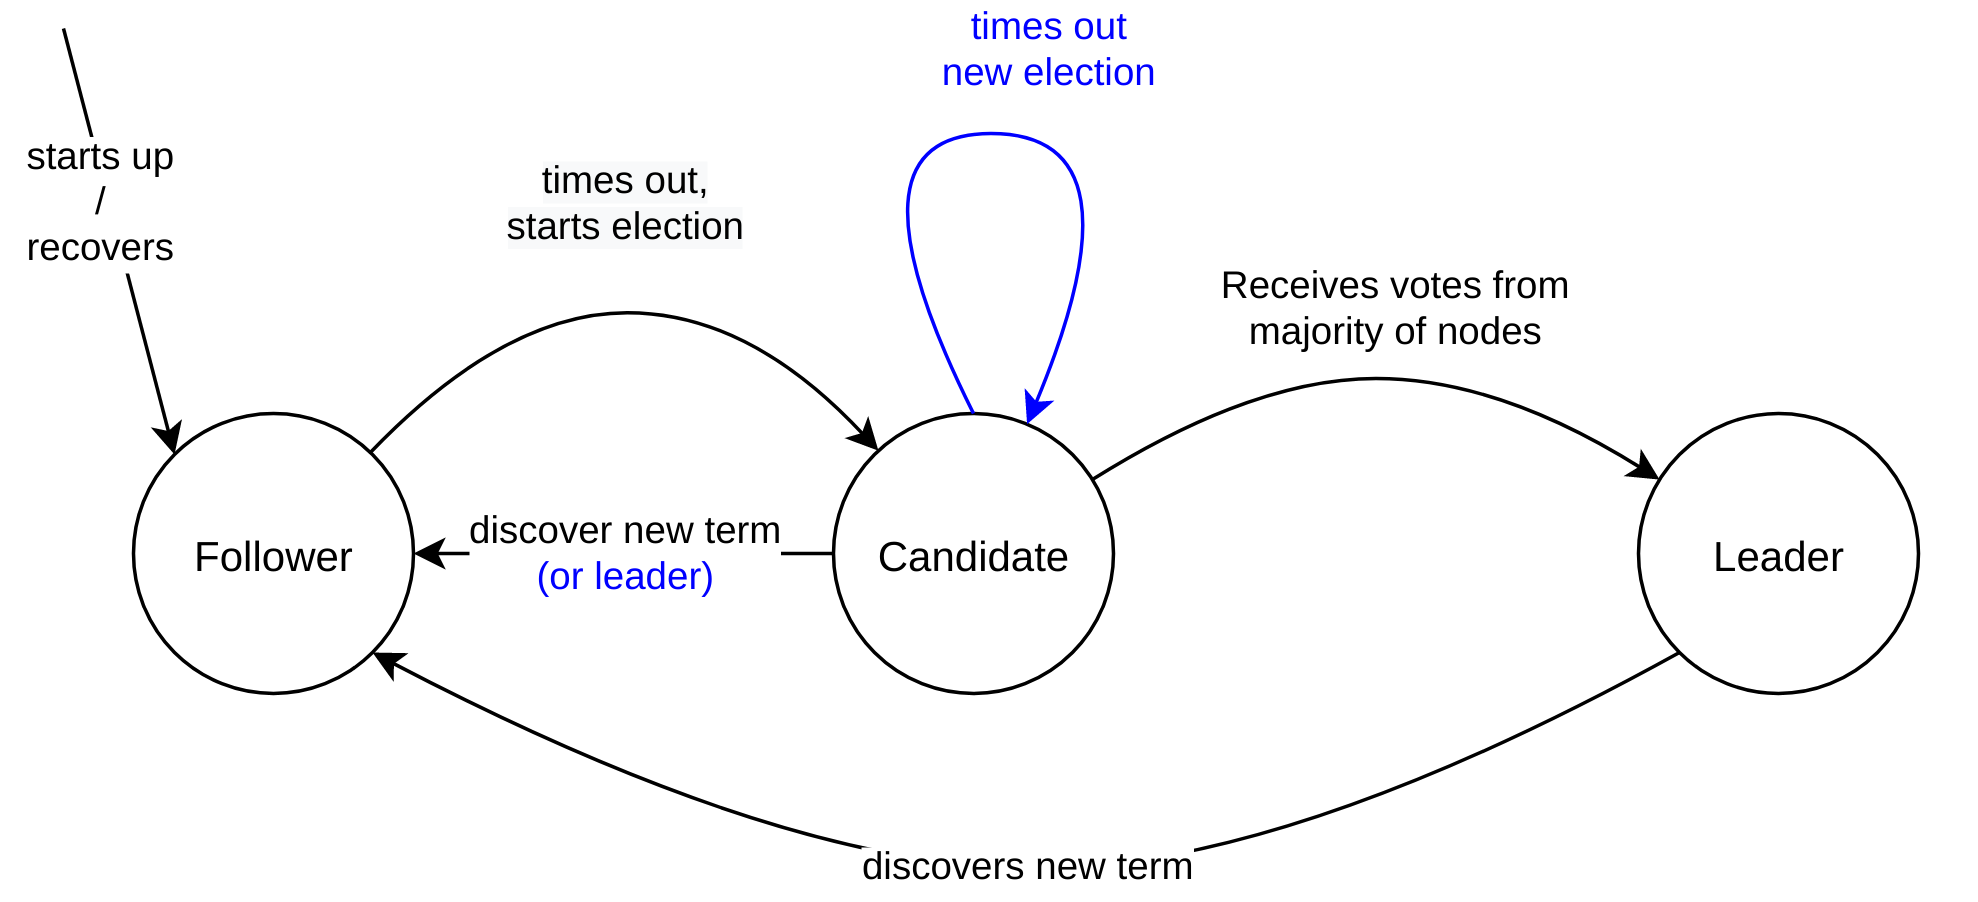
\includegraphics[width=0.8\textwidth]{img/roles-transitions.png}
  \caption{Role transitions between the nodes for Paxos \& Raft. The blue transitions are for Raft only.}
  \label{fig:roles-transitions}
\end{center}
\end{figure}

As Figure~\ref{fig:roles-transitions} indicates,
a node may be a \textit{Follower}, a \textit{Candidate} or a \textit{Leader}.
The \textit{Follower} is responsible for remote procedure calls which
also includes voting for a leader. A node is only in the \textit{Candidate} phase when trying to become a leader.
The \textit{Leader} is responsible for appending logs to its state machine after
asked other nodes to do it.

Initially, all nodes are followers.
Each node remains as a follower until
it believes the leader has failed, at which point it becomes a candidate. If a node successfully becomes a leader, the others become followers which follow the append operations broadcasted by this leader. Each node also keeps a number,
named \textit{term} which is used to perform leader elections during
the operation of the system. When a node receives any message,
it first checks the term of the sender; if the sender's term is
greater than local term, the node updates its term to the greater one
and reacts according. If the two terms are equal,
the node reacts directly. Otherwise, if the sender's term is
lower than the local term, it responds to the sender with
its greater term and changes itself to be a candidate trying to become a leader.

\subsubsection{Log Entry}
A log entry is a pair of operation an term. Operations are sent to
the leader in log entries from followers. The leader is responsible for
receiving the log entries and maintaining the consistency of the whole system.
When the leader receives a log entry, the leader asks followers to
append the log entry. If a majority of followers respond
with confirmation of the appending, the leader then records
the operation to its state machine. To ensure the order of logs,
in this phase, a follower can only append a log when
its prior log or logs are identical to the leader's log.
And a follower can only respond its confirmation after
it recorded the appending to its state machine.

\subsubsection{Leader Failures Handling}
Despite the similarities of Paxos and Raft,
they use different strategies to handle leader failures.

For Paxos, a follower becomes a candidate if it fails to receive any message
from the leader for a specific time. Its term will be increased to the next
such that $\mathrm{term} \mathrm{mod} n = s$ where $\mathrm{term}$ is the next term,
$n$ is the count of nodes and $s$ is the node id of this candidate.
During this election, this candidate must ensure
it has all the previous logs before it becomes a leader.
Thus, followers that vote for this candidate should respond with
a election message which also includes all the log entries that
the follower has after the candidate’s commit index.
The candidate reviews all the log entries it receives,
comparing them with its own logs. If the candidate has a same log,
it updates its own log with the new term.
If the same index has multiple log entries, the candidate uses
the greatest and newest term to update the conflict log.
After all log entries have been checked, the candidate can then
become a leader and start to replicate the log entries to followers.

For Raft, a node will also become a candidate and increase its term if
it fails to receive any message from the leader for a specific time.
It asks other nodes to vote for it with its new term after becoming a candidate. Any node receiving the request will check if the requested term is greater than the one it has locally. If the requested term is indeed greater and the node did not vote for a candidate previously in the same term,
the node votes for the requested candidate.
After a candidate receives confirmations from a majority,
it becomes a leader. Because log entries of Raft are in order,
a node need only check its last log entry, making the election and log replication more efficient.
However, the leader cannot record operation using the term which
it used for the election for safety reason.
As there may be multiple candidates trying to become a leader at the same time with
the same term, it is possible that no candidate can get votes for a majority.
If this happens, a new election with a new term will be started by a candidate.

\subsubsection{Summary}
Overall, Raft is easier to understand and implement. However, in essence, the approaches of Paxos and Raft is quite similar. The main difference between them is that the process of election of the leader in Raft is simpler.
Specifically:

\begin{enumerate}
    \item When choosing a leader, Paxos divides terms between servers.
Conversely, in Raft, each follower can be a candidate in any term,
but each follower can only vote for one candidate; the candidate with the majority votes will become the leader.
    \item In Paxos, followers can vote for any candidate,
even if the log entries in that candidate are not up-to-date.
However, followers in Raft only vote for a candidate
whose log is at least as up-to-date as that follower's.
This ensures the log of the leader is as up-to-date as the most of followers'
    \item Once a leader is elected in Paxos, the leader replicates the log entries in the current term, just as the log entries come from the leader's term. However, in Raft, the leader replicates the log entries to other servers without changing the term.
\end{enumerate}

%%%%%%%%%%%%%%%%%%%%%%%%%%%%%%%%%%%%%%%%%%%%%%%%%%%%%%%%%%%%%%%%%%%%%%%%%%%%%%%%

\section{Paxos Algorithm Details} \label{sec:paxos}

In distributed computing, processes communicate and cooperate with each other to coordinate actions \cite{fischer1983consensus}. Paxos is designed to achieve consensus which ensures that only a single value be chosen from a set of values proposed by some processes. After being chosen, this value is also available to be learnt by all processes. There are many variants based on Paxos \cite{lamport2001paxos} including Fast Paxos \cite{fastpaxos}, S-Paxos \cite{spaxos}, OpenReplica \cite{openreplica} and Ring Paxos \cite{ringpaxos}.

The following content of this section explains the Paxos algorithm based on
\cite{fischer1983consensus}. In their work, they make two assumptions and then give principles to solve the consensus problem.
These principles require a proposal approach in which
each proposal has an ordered number \textit{n} and a proposal value \textit{v}.
The principles also require three classes of agents which
are proposers, acceptors and learners.
There are two phases when choosing a value.
\textit{Phase 1} is to \textit{prepare} a proposal by requesting a majority of acceptors.
\textit{Phase 2} is to ask the majority to \textit{accept} this proposal.
In this phase, any acceptor among the majority can either
accept or decline the \textit{accept} request.

\subsection{Assumptions}
The Paxos algorithm makes two assumptions, detailed below.
\begin{quote}
  \begin{assumption}{1}{F}\label{as:1}
    Processes run asynchronously.
    Processes run at arbitrary speed, may crash and may rejoin.
  \end{assumption}
  \begin{assumption}{2}{F}\label{as:2}
    Message passing is used for processes to communicate with each other.
    It takes arbitrarily long to deliver messages.
    Messages may be lost, may be duplicated, will never be corrupted.
  \end{assumption}
\end{quote}
\subsection{Principles}

The principles are given here and will be applied later,
\begin{quote}
  P1. The first proposal that an acceptor received must be accepted.
  \begin{quote}
    a. A proposal numbered \textit{n} can only be accepted
      iff the acceptor has not responded to any \textit{prepare} request
      with a greater number than \textit{n}.
  \end{quote}
  P2. After chose a proposal with value \textit{v},
    every higher-numbered and chosen proposal has value \textit{v}
    \begin{quote}
      a. After chose a proposal with value \textit{v},
        any proposer should issue the higher-numbered proposal with value \textit{v}.

      b. If a proposal is issued with value \textit{v} and number \textit{n} ,
        there must be a majority of acceptors such that either
          \begin{quote}
            (i) no acceptor in the majority has accepted
              any proposal numbered less than \textit{n}, or

            (ii) \textit{v} is the value of the proposals which
            have smaller \textit{n} comparing with the
            accepted \textit{n}  by the majority.
          \end{quote}
  \end{quote}
\end{quote}

\subsection{Three Agents}
To achieve consensus, there are three classes of agents---proposers, acceptors and learners.
When a process proposes a proposal, it is included in the class of proposers.
When a process receives requests from any of the proposers,
it is then included in the class of acceptors.
And when a process learn a chosen value, it is included in the class of learners.
These three cases can happen simultaneously, i.e.
a process can propose, receive requests or learn a chosen value at the same time.
Thus, the three classes of agents are not mutually exclusive for a single process.

\subsection{Implementation}

\subsubsection{Choosing A Value} \label{Choosing}
The Paxos algorithm \cite{lamport1998part} chooses a leader
from the processes of assumption \ref{as:2}.
This leader is the leader of the class of proposers and
also the leader of the class of learners at the same time.
A proposal is tagged with an ordered number \textit{n} and a value \textit{v}.
The proposal will be passed from one proposer to the leader.
This leader is in charge of requesting a majority of accepters to ask for acceptance.
The majority can be generated by the algorithm \cite{keidar2001cost}.

A proposal will be requested two times to finally be chosen.
Upon the first request, named the \textit{prepare} request,
an acceptor should respond to the proposer with a \textit{promise} respond.
Once get \textit{promise} respond from a majority
(this majority could be different from the requested one),
the proposer leader requests each \textit{promised} acceptor in the majority
with an \textit{accept} request to confirm the acceptance of this proposal.
The acceptor which receives this \textit{accept} request will
accept this proposal based on $P1^a$. And no matter whether it accepts it or not,
it should respond to the proposer to confirm its reaction.
If a proposal was accepted, i.e. a value was chosen, it then can be learnt by learners.

\subsubsection{Learning a Value}
There are three easy approaches to learn a value.
The first is in \textit{Phase 2}; when acceptors accept a value,
they can respond to all the learners.
This is immediate but requires a response number at
the product of the number of learners and the number of acceptors.
The second approach is for acceptors to respond only to the leader of learners.
However, this is unreliable because of assumption \ref{as:2}.
Finally the third is to have a set of leaders of learners
combining the benefits of the other approaches without lots of message passing.

The three ways above are all passive from the perspective of a learner.
If a learner wants a chosen value itself, it can generate another agent (a proposer) to propose a value using the above algorithm to get the desired value.

\subsection{Issues}
Because of assumption\ref{as:1} and the use of a quorum of acceptors
\cite{jalili2014practical}, acceptors have to handle messages sequentially.
Thus, performance hiccups may occurs when it takes time for slower acceptors to catch up.

Paxos has several significant shortcomings.
The first one is that the original paper is very vague
and few people can fully understand it \cite{conf/usenix/OngaroO14}.
To describe the Paxos algorithm, Lamport described a parliament on a small island
in Greece \cite{lamport1998part}.
Although Lamport later published a paper trying to simplify the description
of the algorithm \cite{lamport2001paxos}, understanding Paxos is still a significant challenge.
Another drawback of Paxos is that it does not provide a good foundation for
building practical implementations \cite{conf/usenix/OngaroO14}.
The description of the algorithm in Lamport's paper is
just an algorithm for a single decree. Lamport mentioned the solution to
implement Multi-Paxos, but many details are not sufficiently provided,
which leads to the existing implementation of Paxos being
based on the implementers' own understandings.
As a result, practical systems usually vary widely.

%%%%%%%%%%%%%%%%%%%%%%%%%%%%%%%%%%%%%%%%%%%%%%%%%%%%%%%%%%%%%%%%%%%%%%%%%%%%%%%%

\section{Raft Algorithm Details} \label{sec:raft}

The Raft algorithm was proposed in 2014 \cite{conf/usenix/OngaroO14} as an alternative to the (Multi-)Paxos algorithm, with the intent of being more understandable and easier to implement in a practical system. The highlight of the Raft algorithm is that it adopts an engineering thinking---it simplifies the model of the design according to the requirements in practical applications and modularises the process of the algorithm. From the perspective of performance and security, the authors state that Raft algorithm is also almost the same as Paxos \cite{conf/usenix/OngaroO14}.

\subsection{Roles}
  Nodes in the Raft algorithm can perform one of three roles, as detailed below.

  \subsubsection{Follower}
  All nodes are followers upon starting. Followers are completely passive; they can only respond to incoming messages. If a client's message is sent to a follower, the Raft algorithm specifies that it be rejected and the client redirected to the leader (see below). A follower may transition to a leader through an election under certain conditions. Such conditions are detailed in \S\ref{sec:raft-leader-elec}.

  \subsubsection{Leader}
  There can be only one Leader in the entire cluster at the same time. The leader handles all client interactions.

  \subsubsection{Candidate}
  The candidate state is a transitional state between the follower and leader states. When a follower becomes a candidate, an election will be held. The candidate who wins the election will become the new leader.

\subsection{Protocol}
In the Raft algorithm, time is divided into terms \cite{conf/usenix/OngaroO14}. Terms are each identified with a number which increments monotonically as successive terms arise. Each term starts with an election. If the election is successful, the chosen leader will serve for the rest of the term, which means that only one leader can be elected in a given term. Should the election be unsuccessful, then the candidate simply starts a new term. Each node in the cluster maintains the value of the current term number which should be stored reliably. The purpose of the term and term number is to allow nodes to identify information that is out of date.

In order for followers to continuously be aware of the active leader in the cluster, they expect to receive heartbeat messages from the leader regularly. If a follower's timeout of for an heartbeat message elapses, it assumes that the leader has crashed and will start a new election. This timeout is often much longer than the expected propagation time of the message across the network.

There are only two types of RPCs between nodes in the Raft algorithm (not including the RPC to handle client requests):
\begin{itemize}
  \item \textbf{RequestVote RPC}: invoked by candidates to gather votes \cite{conf/usenix/OngaroO14} from other nodes.
  \item \textbf{AppendEntries RPC}: invoked by the leader to replicate log entries \cite{conf/usenix/OngaroO14}.
\end{itemize}

  \subsubsection{Leader Election} \label{sec:raft-leader-elec}
  When a node begins an election, the first thing it does is to increment its current term number. The node then converts itself from follower state to candidate state. To win the election, the node must receive votes from a majority of nodes in the cluster. The node votes for itself, then sends RequestVote RPCs to all other nodes and retries this process until either:
  \begin{itemize}
    \item It receives votes from a majority of nodes in the cluster, in which case it wins the election and becomes the leader; or
    \item It receives an RPC from a leader, in which case another candidate has won the election and the node becomes a follower; or
    \item The election timeout elapses, which means that no one has won the election. The node will then increment the term number and start a new election.
  \end{itemize}

  To ensure safety, each node can only give out at most one vote in a term. This guarantees that only one candidate can obtain votes from a majority in the same term; thus, only one candidate can win the election. Also, to prevent live lock of the election (i.e. candidates perpetually competing against each other), the election timeout for each node is randomised.

  \subsubsection{Log Replication}
  Once a leader is elected, it receives all client's request messages. These messages contain a command to be executed by the replicated state machine. The leader creates a log entry for each request from the clients. Apart from a command, each log entry also contains an index number in the log and a term in which the log entry was first created. Each log entry is committed if it is known to be stored in the logs of a majority of the nodes.

  When the leader receives a command from a client, it appends the command with the current term number and index number to its log. Then, the leader sends \texttt{AppendEntries} RPCs to all followers. Once a new log entry is committed, the leader passes the command to its state machine and notifies all followers of this new log entry. When the followers receive these RPCs, they pass the command to their state machine.

  To ensure consistency of logs, each \texttt{AppendEntries} RPC contains the index and the term of the previous log entry. The followers who receive the RPC will reject the request if they do not have the matching log entry. Hence, it is guaranteed that a new entry only be accepted if the logs match in their previous entry. If a given log entry is committed, all preceding log entries are also committed.

  At the beginning of a new leader's term, the old leaders may have left some log entries that are partially replicated. The way that the Raft algorithm solves this problem is to force all followers to duplicate its log, which will also force all followers to discard inconsistent log entries and fill in whose which are missing. The leader maintains a value \texttt{nextIndex} for each follower, which marks the index of the next log entry to send to that follower. When the \texttt{AppendEntries} consistency check fails, it decrements \texttt{nextIndex} and retries until the follower's log is repaired.

  \subsubsection{Safety}
  If a leader has decided that a log entry is committed, then that entry should be present in the logs of all future leaders \cite{conf/usenix/OngaroO14}. To guarantee this, the algorithm picks the candidate to win the election such that it has the log that is most likely to have all the entries that have been committed. Hence, candidates must include their respective log information in their \texttt{RequestVote} RPCs including index and term of the last log entry. A voting server must deny the vote if its log is more complete.

  Another safety issue is that if a leader crashes while replicating logs, the new leader will not know whether the last log entry of the previous leader has been committed or not. To solve this problem, a new commitment rule must apply---for a leader to decide whether an entry is committed, in addition to the previous rule, at least one new entry from the leader's term must also be stored on the majority of servers.

  \subsection{Future Improvements}
  \subsubsection{Pre-vote}
  Network partitions can lead to a wide gap between the data of some nodes and the latest data of the cluster. Hence, the term can become very large due to continuous attempts to start elections. After the network has recovered, the leader will step down when it tries to replicate its log to these nodes and then discover larger term numbers. This situation can be avoided by introducing a pre-vote---before changing to candidate state, followers first communicate with other nodes in the cluster to obtain information about whether the leader is alive. If the current cluster has a leader alive, the follower will not become a candidate. Thus, the term number will not increase.

  \subsubsection{Leader stickiness}
  One drawback of the Raft algorithm is the potential for leader flip-flopping in some corner cases due to a network partition. Consider the following scenario in Figure \ref{fig:network-partition-example}. Initially, node 1 is the leader and nodes 2 and 3 are followers. From a certain moment, the connection between nodes 1 and 2 is broken. During this specific time period, there is no request from the client (which means nothing will be added to leader's log). As the election timeout triggers node 2 to start a new election, it obtains votes from node 2 and itself, making it become the new leader. Node 1 will learn this change from node 3 and then step down. However, node 1 cannot receive heartbeat messages from node 2, which will lead to a new election and node 1 will then become the leader. This flip-flopping continues forever until the communication between nodes 1 and 2 has recovered. The idea of leader stickiness is intuitive; followers should reject a \texttt{RequestVotes} RPC if it considers the current leader to be working properly. This ensures in the scenario given, node 2 will never win the election.

  \begin{figure}[htp]
    \centering
    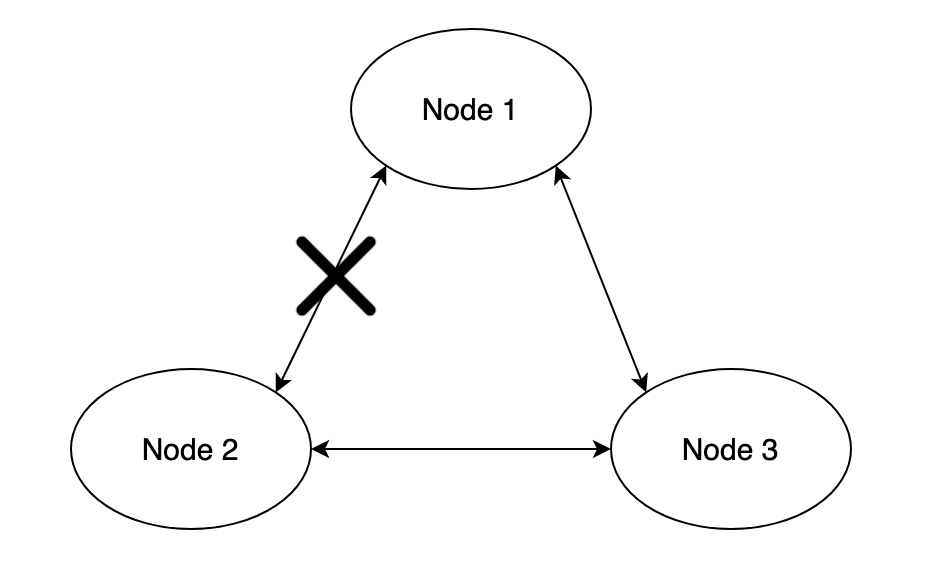
\includegraphics[width=0.5\textwidth]{img/network-partition-example.png}
    \caption{Example for leader stickiness}
    \label{fig:network-partition-example}
  \end{figure}
%%%%%%%%%%%%%%%%%%%%%%%%%%%%%%%%%%%%%%%%%%%%%%%%%%%%%%%%%%%%%%%%%%%%%%%%%%%%%%%%

\section{Application and Algorithm Implementation} \label{sec:application}
We implement a distributed key-value database in Java using the Raft consensus algorithm. Although Paxos is the dominant consensus algorithm in the industry, Raft is selected due to its strong focus on being an understandable algorithm. Further, unlike Paxos, Raft is a \textit{continuous} algorithm which we deem to be more suitable for our application. Although there is a variant of Paxos which is similarly continuous (Multi-Paxos), we find the Raft algorithm to be less complex to implement.

Our key-value database takes the form of a \texttt{HashMap} which is replicated (as opposed to sharded) across all nodes in the cluster. Due to this replication, it is crucial that our system remain consistent over time; key-value pairs should match across different nodes. Hence, we solve the problem with the aid of consensus.

\subsection{Architecture}
All nodes in our system share the same architecture, shown in Figure \ref{fig:uml}. Communication between nodes is achieved by Java Remote Method Invocation (RMI). Below, we discuss the rationale behind our design decisions.

\texttt{NodeImpl} is the main class of a node, holding references to a \texttt{RaftLog} object and an object corresponding to the current state of the node (i.e. follower, candidate or leader). The class implements \texttt{INode} (which extends \texttt{Remote}) to be able to receive RMI calls from other nodes---the \texttt{requestVote} method is called by candidate nodes and the \texttt{appendEntries} method is called by the leader. Additionally, the class implements \texttt{IClientInterface} to be able to receive RMI calls from clients.

However, \texttt{NodeImpl} does not hold a direct reference to the \texttt{StateMachine} object. Instead, the reference to the state machine (which contains the \texttt{HashMap} with the state of the key-value database) is held by the \texttt{RaftLog} object instead. This design decision was made as a safeguard against system inconsistencies which could possibly arise from unintentional manipulation of the state machine. \texttt{NodeImpl} should not concern itself with the state machine; its focus should rather be on appending and committing \textit{log entries}. The \texttt{RaftLog} object takes responsibility for applying the correct log entries to the state machine, based on whether they have been successfully committed.

The three different states in which a node can be correspond to three classes---\texttt{CandidateState}, \texttt{FollowerState} and \texttt{LeaderState}---to segregate behavioural differences based on state and avoid the need to repeatedly check the state that the node is in. These classes all extend \texttt{AbstractState} which encapsulates common parameters such as the minimium and maximum election timeout.

We made a conscious decision to make attributes of \texttt{AbstractState} such as \texttt{currentTerm} and \texttt{votedFor} static. Since the application is distributed, all nodes run on separate machines (and hence, different JVMs). Thus, there is no issue with making these attributes static. By doing so, we have the benefit of the values being carried over seamlessly when a node changes state; the attributes are not tied to a specific object.

\begin{figure}[htp]
  \centering
  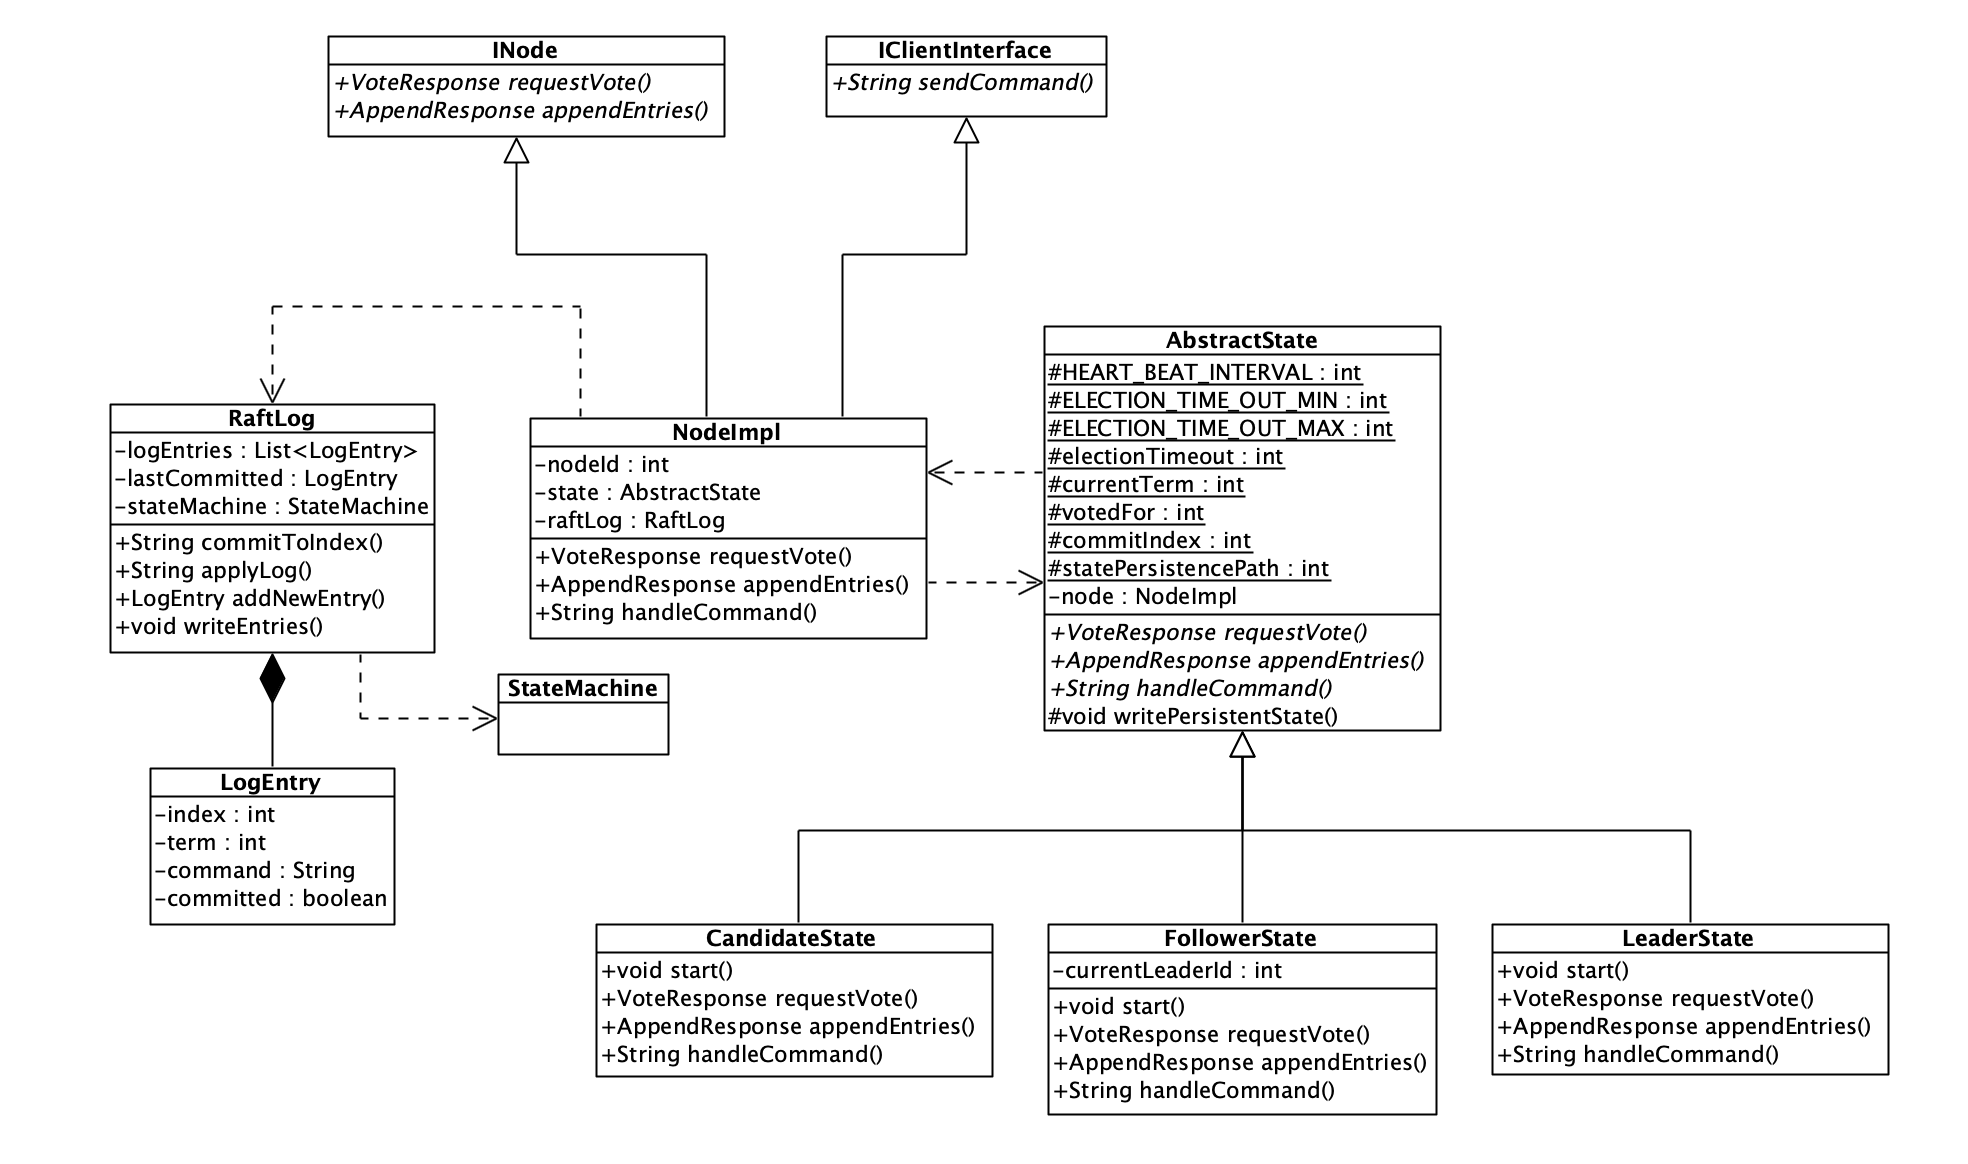
\includegraphics[width=1\textwidth]{img/class-diragram.png}
  \caption{Class Diagram}
  \label{fig:uml}
\end{figure}

\subsection{Operational Details}
The system is made available by starting at least half the nodes in the cluster. All nodes have a configuration file detailing:
\begin{itemize}
    \item The ID of the node
    \item For every other node in the cluster:
    \begin{itemize}
        \item Its ID
        \item Its IP address and port
    \end{itemize}
\end{itemize}
Upon starting a node, it attempts to connect to all other nodes listed in the configuration file. In the event that it can't connect to a particular node, it tries again periodically for up to 30 seconds before continuing to the normal state of operation. As per the Raft algorithm specification, all nodes start in the follower state. The transition from one state to another is handled by the incumbent state. For instance, should a leader node receive an \texttt{appendEntries} RMI call containing a higher term than its own, its \texttt{state} object (i.e. \texttt{LeaderState} object) will handle cleanup operations (such as ensuring that periodic heartbeats no longer be sent) and instantiate a new \texttt{FollowerState} object, reassigning the \texttt{state} attribute of the \texttt{NodeImpl} object to the newly created object.

During operation, changes made to the log are written to persistent storage. This ensures that upon crashing and recovering, a node can simply read the previous state of the log. Note, however, that this is not a requirement of the algorithm. Indeed, a node in our system can recover successfully even if all previous log entries are lost (e.g. due to storage corruption). Nonetheless, recovery is made more efficient if the log is written to persistent storage, since fewer log entries need to be sent from the leader in order for the recovered node's log (and hence, state machine) to catch up with that of the system.

\subsection{Algorithm Enhancement}
During the development of our Raft implementation, we observed that an enhancement to the algorithm could be made. Specifically, we augmented the algorithm such that a client is able to issue a request to any correct node in the cluster, not only the leader.

In the extended version of their paper, Ongaro and Ousterhout (the authors of the Raft algorithm) detail that only the leader node is required to handle client requests. As such, they specify that clients should only contact the leader; should a client connect to another node, the node will reject the request and inform the client of the most recent leader it knows.

This restriction leads to unnecessary inefficiencies. For instance, when a client first starts up, it selects a server randomly. This is unlikely to be the leader so it must issue another request. The same is true in the event that the leader crashes---in this case, the request would timeout and the client would similarly select a server randomly, again unlikely to be the leader.

The need for a client to issue duplicate requests as detailed above is easily mitigated by a minor addition to the algorithm. In our implementation, should the client contact a non-leader node, the node simply forwards the request directly to the leader, acting somewhat like a proxy. In doing so, the non-leader node invokes the same method of the leader that clients would invoke. Thus, to the leader, there is effectively no difference between receiving an application request from a client and one from another node. Upon receiving the result from the leader, the non-leader node will simply pass it on to the client. Hence, requests are handled seamlessly and the client need not concern itself about who the leader is.

%%%%%%%%%%%%%%%%%%%%%%%%%%%%%%%%%%%%%%%%%%%%%%%%%%%%%%%%%%%%%%%%%%%%%%%%%%%%%%%%

\section{Application Domains and Future Directions}\label{sec:future}
Consensus algorithms that guarantee partition-tolerance and consistency such as Paxos and Raft can be applied to:
\begin{itemize}
    \item Distributed duplicated transaction systems
    \item Managing leader node for managing and scheduling distributed tasks (detailed below)
    \item Synchronisation of replicas in the state machine and ensuring consistency among them
\end{itemize}

This kind of algorithm is widely used in the industry and supports many real-world applications and systems. For example, Docker Swarm---a well-known container orchestration tool---uses the Raft algorithm to ensure that all the manager nodes that are responsible for managing and scheduling tasks in the cluster store the same consistent state. In this way, any manager node can pick up the tasks and restore to a stable state when the leader manager crashes. Additionally, Google's Chubby \cite{burrows2006chubby}---a lock service for loosely-coupled distributed systems---uses Paxos to maintain the consistency of its replicas in its fault-tolerant log. Zookeeper uses its own improvement of Paxos, called ZAB
\cite{junqueira2011zab}, to propagate the corresponding incremental state changes to backup processes.

Currently, voting-based consensus algorithms are largely mature and stable. The latest research in this field mainly surrounds improving the traditional algorithms to tailor them towards specific applications. Today, most research regarding consensus focuses on proof-based algorithm relating to blockchain. While this can be largely attributed to the recent advent and proliferation of cryptocurrencies, proof-based consensus algorithms can be applied in other ways also. For example, a blockchain-based approach can be used to solve some security problems surrounding the Internet of Things (IoT) \cite{zhang2020blockchain}.

\bibliographystyle{ieeetr}
\bibliography{main}

\end{document}
